\documentclass[british]{article}
\usepackage[utf8]{inputenc}
\usepackage[british]{babel}% Recommended
\usepackage{csquotes}% Recommended

\usepackage[sorting=nyt,style=apa]{biblatex}

\addbibresource{~/Tex/library.bib}
\usepackage[toc,page]{appendix}
\usepackage[margin=1in]{geometry}

\usepackage{amsmath}
\usepackage{graphicx}
\usepackage{listings}
\usepackage{enumerate}
\newcommand{\code}[1]{\texttt{#1}}
\newtheorem{defin}{Definition}
\newtheorem{prop}{Proposition}
\newtheorem{col}{Corollary}
\newtheorem{thm}{Theorem}
\setlength{\parskip}{1em}
\usepackage{placeins}

%Default fixed font does not support bold face
\DeclareFixedFont{\ttb}{T1}{txtt}{bx}{n}{12} % for bold
\DeclareFixedFont{\ttm}{T1}{txtt}{m}{n}{12}  % for normal

% Custom colors
\usepackage{color}
\definecolor{deepblue}{rgb}{0,0,0.5}
\definecolor{deepred}{rgb}{0.6,0,0}
\definecolor{deepgreen}{rgb}{0,0.5,0}

\usepackage{listings}

% Python style for highlighting
\newcommand\pythonstyle{\lstset{
		language=Python,
		breaklines=true,
		frame=single,
		numbers=left,
		tabsize=2,
		basicstyle=\ttm,
		otherkeywords={self},             % Add keywords here
		keywordstyle=\ttb\color{deepblue},
		emph={MyClass,__init__},          % Custom highlighting
		emphstyle=\ttb\color{deepred},    % Custom highlighting style
		stringstyle=\color{deepgreen},
		frame=tb,                         % Any extra options here
		showstringspaces=false            % 
}}


% Python environment
\lstnewenvironment{python}[1][]
{
	\pythonstyle
	\lstset{#1}
}
{}

% Python for external files
\newcommand\pythonexternal[2][]{{
		\pythonstyle
		\lstinputlisting[#1]{#2}}}

% Python for inline
\newcommand\pythoninline[1]{{\pythonstyle\lstinline!#1!}}

\title{CS4402 - Practical 1: Bombastic}
\author{170008773}
\date{\today}

\begin{document}
\maketitle


\begin{abstract}
 The planning of sequences of moves is a common problem in constraint solving, having applications from problems like scheduling to route planning. To be able to solve these problems efficiently they have to be modelled in such a way that solvers can work with the data efficiently. Here it is critical to note that the way these problems are modelled can have potentially huge impacts in how efficiently they can be solved. As an exercise in constraint modelling I have modelled the game Bombastic in Essense Prime. In this report I will detail the design choices, the testing of the model, and the results of benchmarking the model with different levels of optimisation performed by the solver. 
\end{abstract}

\section{Problem description}
\label{problem}
\subsection{The game}
Bombastic is played on a $N\times M$ grid of cells. The cells in this grid can either be \code{dead}, \code{ice}, or \code{normal}. \code{dead} cells cannot be entered by anything, and other cells can accomodate at most one block or the avatar. For simplicities sake we assume that every grid is surrounded by a wall of dead cells. On this grid there is an avatar and one or more blocks and a number of goals, \texttt{equal to the number of blocks}. The objective of the avatar is to walk around the gird and push the blocks around until all blocks are at a goal. In this scenario we are not interested in which block ends up at which goals.  


\subsection{Avatar logic}
The avatar is allowed to move around the grid, moving the cell it is currently occupying to any of the adjacent cells that are not dead. The avatar is only allowed to move purely horizontally or vertically (i.e. not at the time) and not moving is also disallowed.  The player is allowed to move onto an ice cell, however when it moves off that cell again, the ice will crack, turning the cell into a dead one. 


\subsection{Box logic}
The avatar can move blocks by moving into their square. This will move the block one square in the direction the avatar is travelling in. This is only allowed if the cell the block is moving into is not dead and does not contain another block.

\subsection{Objectives}
Given the grid layout, the positions of the blocks, the position of the goals, and the initial position of the avatar, the objective is to find a sequence of legal moves that move all the blocks to a goal. In this instance the number of moves is provided. So the problem is to find whether there is a sequence of the given length that satisfies all the objectives. 


\section{Modeling the problem}
I will now detail how the assignment was setup, the majoor modelling ethos used and the new instances I designed. 
\label{model}
\subsection{Setup}
In this instance I was required to use the modelling language \code{Essence prime} in conjunction with the constraint solver Savile Row. I was also provided with the decision variables, their domains and several sets of parameters to test the system. I was required to add the constraints to accurately model the problem and solve the provided instances, as well as design several new instances. 

\subsection{Modelling decisions}
\paragraph{Redundancy}
As mentioned previously , the way that the problems are modelled can have big impacts in how efficiently they are solved. The less constraints there are to check, the less work the solver has to perform. In this we have a decision to make. So there is an incentive to make the constraints as simple and as small in number as possible. On the other hand however these models, even ones that are well constructed, can be very complex to interact with on a human level. To mitigate this, extra constraints that overlap with, or even imply other constraints as sanity checks. Ultimately, these are judgement calls as either extreme is likely to cause problems. In the modeling of this problem I opted to lean towards redundant constraints, feeling that an extreme focus on performance was not needed considering the scope of the project. 

\paragraph{Elegance} In contrast to redundancy, it benefits both human and machine to simplify the constraints as much as possible. This practice can make the model more understandable to humans and easier to solve for the machine. Where possible we attempted to make the constrains as small as possible, trying to eliminate conjunctions or disjunctions where possible. So too did we try to use existential quantifiers where possible because these are more efficient than universal quantifiers. 

\subsection{Model description}
\paragraph{Overview} The model is rounghly devided into four parts: Initialisation, Game logic, Avatar logic and Box logic, each of which I will discuss below. 

\paragraph{Initialisation} This is fairly straght forward. We are given the initial positions for the goals, the blocks, the map layout and the avatar. In this section we simply loop over all our enviroment variables at time 0 and set them to the initial parameters we recieved. 

\paragraph{Game logic} The game logic seciont is mainly concerned with detailing the end conditions of the game, namely that all the goals must have a block occupying them, and how the cells in the map are or are not supposed to change. Here we chose to add some redundent constraints that state that normal cells stay normal and dead cells stay dead as a sanity check. Finally we state that ice cells crack when the avatar leaves them. Since not moving is disallowed, we did this by checking when the avatar enters the ice cell, and killing the cell in the next step.

\paragraph{Avatar logic} The avatar logic is also relatively straight forward. They cannot enter dead cells, their positioin should be updated using the \code{moveCol} and \code{moveRow} variables and they are only allowed to move one square in either a vertical or horisontal direction. We chose to model with using the sum of the abolute values of them move variables because this semultaniously details which moves are allowed and disallows both diagonal movement and non-movement. 

\paragraph{Box logic} Box movement is the most complicated part of this model since it involves the most variables. Making a block move invoves checking the blocks position, the position of the avatar, the direction the avatar want's to move to and the position that the block itself would move too. Here it is also useful to note that we need to add constraints that blocks are not allowed to move unless pushed by the player, to avoid the solver simply teleporting them to the goals at any point in time. Because this is the most complex part of the model we have opted to leave in the most redundant constraints. For example the constraint that blocks can share a cell would have been enough to ensure that no two blocks can be pushed samiltanously, but since this depends on how the movement of the avatar is checked, we decided add a seperate constraint for this as a sanity check. 


\subsection{Designed instances}
I was also required to design new instances of this problem class. I took this opportunity to design a few instances that can be used to either test specific parts of the modelled logic or some artificially difficult problem to test the performance. They are designed in pairs. Every problem has one paramter file that is solvable and one that isn't so that we can see how the performance compares to comperable problems. To make the process of visualising the results a little easier every impossible version of an instance requests a solution that is 1 step shorter than the shortest solution, even if it is made impossible by other modifications. We will discuss them below. Human readable maps of all the instances are provided in the files. The numbers in the list correspond to the appropriate file name. 
\begin{enumerate}[1)]
	\setcounter{enumi}{9}
	\item This problem is a slight adaptation of the \code{Bombastic1\_1.param}. It is just a single width corridor with two blocks in it. This is designed to test the avatar's inability to push more than one block at the same time.
	\item This is another instance designed to test the ice mechanic. There is a L shaped corridor with an ice cell at the intersection that the avatar starts on and a block and goal in each branch. The possible version removes the ice cell. The impossible version also has a step length less than the possible version. This is not strictly necessary since the impossibility comes form the ice configuration, but this made our naming scheme and subsequently the data collection and visualisation much easier, while it shouldn't change the final outcome.
	\item This problem contains a square of ice in the middle with two single width corridors with a block in them on either end. The possible version has one ice cell replaced with a normal one, making it possible. This instance was designed to test how the solver deals with ice planning, and whether the ice mechanic is done correctly. The impossible version also has a step length less than the possible version. This is not strictly necessary since the impossibility comes form the ice configuration, but this made our naming scheme and subsequently the data collection and visualisation much easier, while it shouldn't change the final outcome.
	\item This instance is a slightly more complicated instance to test the inability of the avatar to push more than one box at a time. It has a small room and two blocks in a row with goals on two sides. This instance requrest a tiny bit of planning, since the avatar will have to walk around the blocks first.
	\item This instance is simply a large open room with no complications. It is designed to test how the solver performs in terms of the length of the solutions and the size of the possible moves while the actual solution is very uncomplicated.
	\item  This instance is a simple adaptation of \code{Bombastic9\_17.param}.  It is identical to the old instance but it has a relatively big empty space added at the bottom that should change nothing about the solution. This was done to test how well the solver would fair if a lot of useless space was added.
\end{enumerate}
	
\section{Emperical evluation}
\label{results}
In this section I will desciribe the testing process I used and discuss the results. 

\subsection{Testing process}
\label{testing}
The testing process was fairly straight forward. In addition to the testing I did while designing the system, I used both the provided instances as well as my own designed instances described above. Like I discussed above I designed some instances with the intention of testing specific aspects of the model and others were designed to test the performance of the model. 

I used a python script to run the solver on every instance with all the optimisation levels and automatically record the data. This data consisted of an instance id, the number of steps of the requested solution, the optimisation level, whether a solution was found and the computation time that the solver took. We measured the computation time in CPU seconds spent in user mode (as described by the bash module \code{time}).  The rest of the data was obtained by a simple parsing of the output f the solver and parameter file. The code for the script can be found in appendix \ref{collection}

\subsection{Results}
\paragraph{Computation per step}
 Because of the intricate nature of constraint problems in general we cannot make precice claims about the space or time complexity of these problems. Therefore we will only discuss the emperical results we have found. In figure \ref{stepsVsCPUSec} you will find the computation times of all the instances that succeeded. I will discuss the relative performance of the possible vs the impossilbe instances shortly. 
 
 As we can see, when the problems are relatively small, the level of optimisation doesn't matter that much. For the simpler problems the least amount of optimisation seems to be best, which makes sense since the extra overhead of optimisation might not be worth it for such small problems. As we increase the length of the requested solution we see that levels 1 and 2 remain roughtly linear. Optimisation level 0 and 3 however, eventualy start exibiting exponential behavour. For level 0 this is what we expected, since the search space grows to fast if we don't make smart optimisations for this.
  
 \paragraph{heavy optimisation} What happens to level 3 however is slightly more counter intuitive. We can explain this as follows. Optimisation is a lot of work and if the search space is less conducive to optimisation then it can waste a lot of effort. We assume that this is what happend since we werent able to model the problem using a lot of global constraints. These global constraints are easiest the optimise away, so the fact that we didn't use them that much might make the heavy optimisation not worht while.
 
 \paragraph{Complexity vs length} It is useful to note however that level 3 outperforms level 0 at a length of 14. This includes one of the designed instances where the instance was just a big wide open room. This was designed to have an artificially long but uncomplicated solution, and here we see that the heavy optimisation is still prefereable to no optimisation.  
\begin{figure}[!ht]
	\centering
	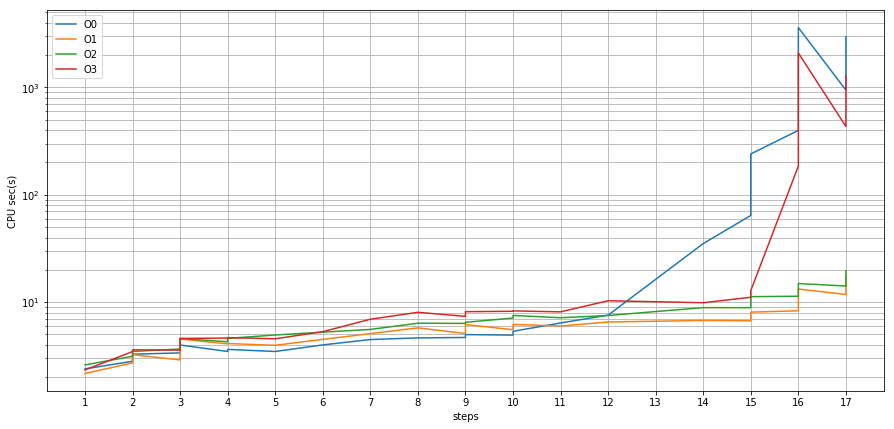
\includegraphics[width=0.9\textwidth]{stepsVsCPUSec}
	\label{stepsVsCPUSec}
	\caption{The number of steps of the requested solution vs. user CPU time. (lower is better)}
\end{figure}


\paragraph{Relative performance of instances} We will now discuss the relative performance of the solver at solving the possible and impossible versions of the same instance. The absolute difference of the computation times of the same instance can be found in figure \ref{idVsCPUSecDiffed}.  
\begin{figure}[!ht]
\centering
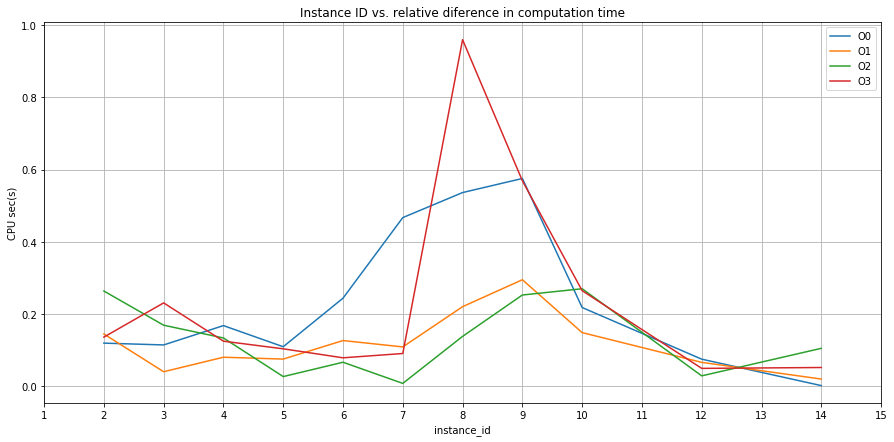
\includegraphics[width=0.9\textwidth]{idVsCPUSecDiffed}
\label{idVsCPUSecDiffed}
\caption{The instance id vs. absolute difference of user CPU time between the possible and impossible variant of every instance. User ids of the designed instances are arranged to have increasing step sizes. (lower is better)}
\end{figure}



%\begin{figure}[!ht]
%\centering
%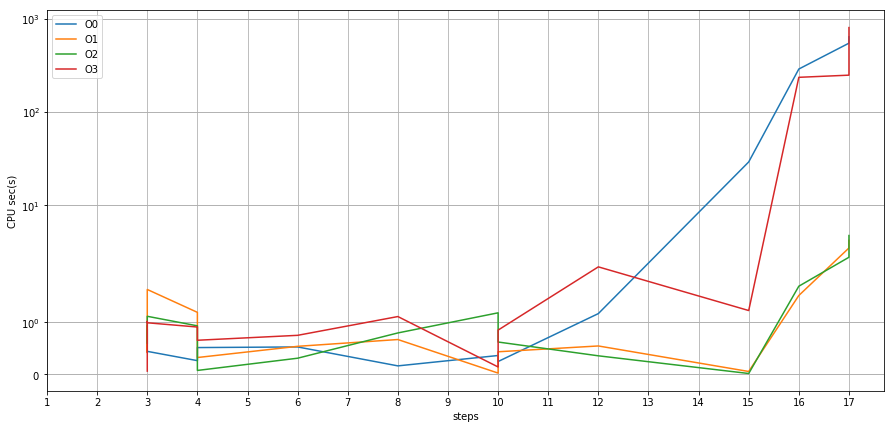
\includegraphics[width=0.9\textwidth]{stepsVsCPUSecDiffed}
%\label{stepsVsCPUSecDiffed}
%\caption{The number of steps of the requested solution vs. absolute difference of user CPU time between the possible and impossible variant of every instance. User ids of the designed instances are arranged to have increasing step sizes.(lower is better)}
%\end{figure}

\section{Conclusion}
\label{conclusion}

word count: 

 \FloatBarrier
 \begin{appendices} 	
 	\section{Data collection script}
 	\label{collection}
 	\pythonexternal{../timer.py}
 \end{appendices}
 

\printbibliography
\end{document}
